\chapter{De practicum omgeving}
\label{chap:omgeving}
%De practicumopdrachten worden gedaan 
De practicumomgeving van dit instructie college bestaat uit een laptop waarbij de BBC:microbit via een USB micro snoertje is aangesloten, zoals te zien is in figuur \ref{fig:aansluiting}.
	\begin{figure}[h!]
	\captionsetup{justification=centering}
	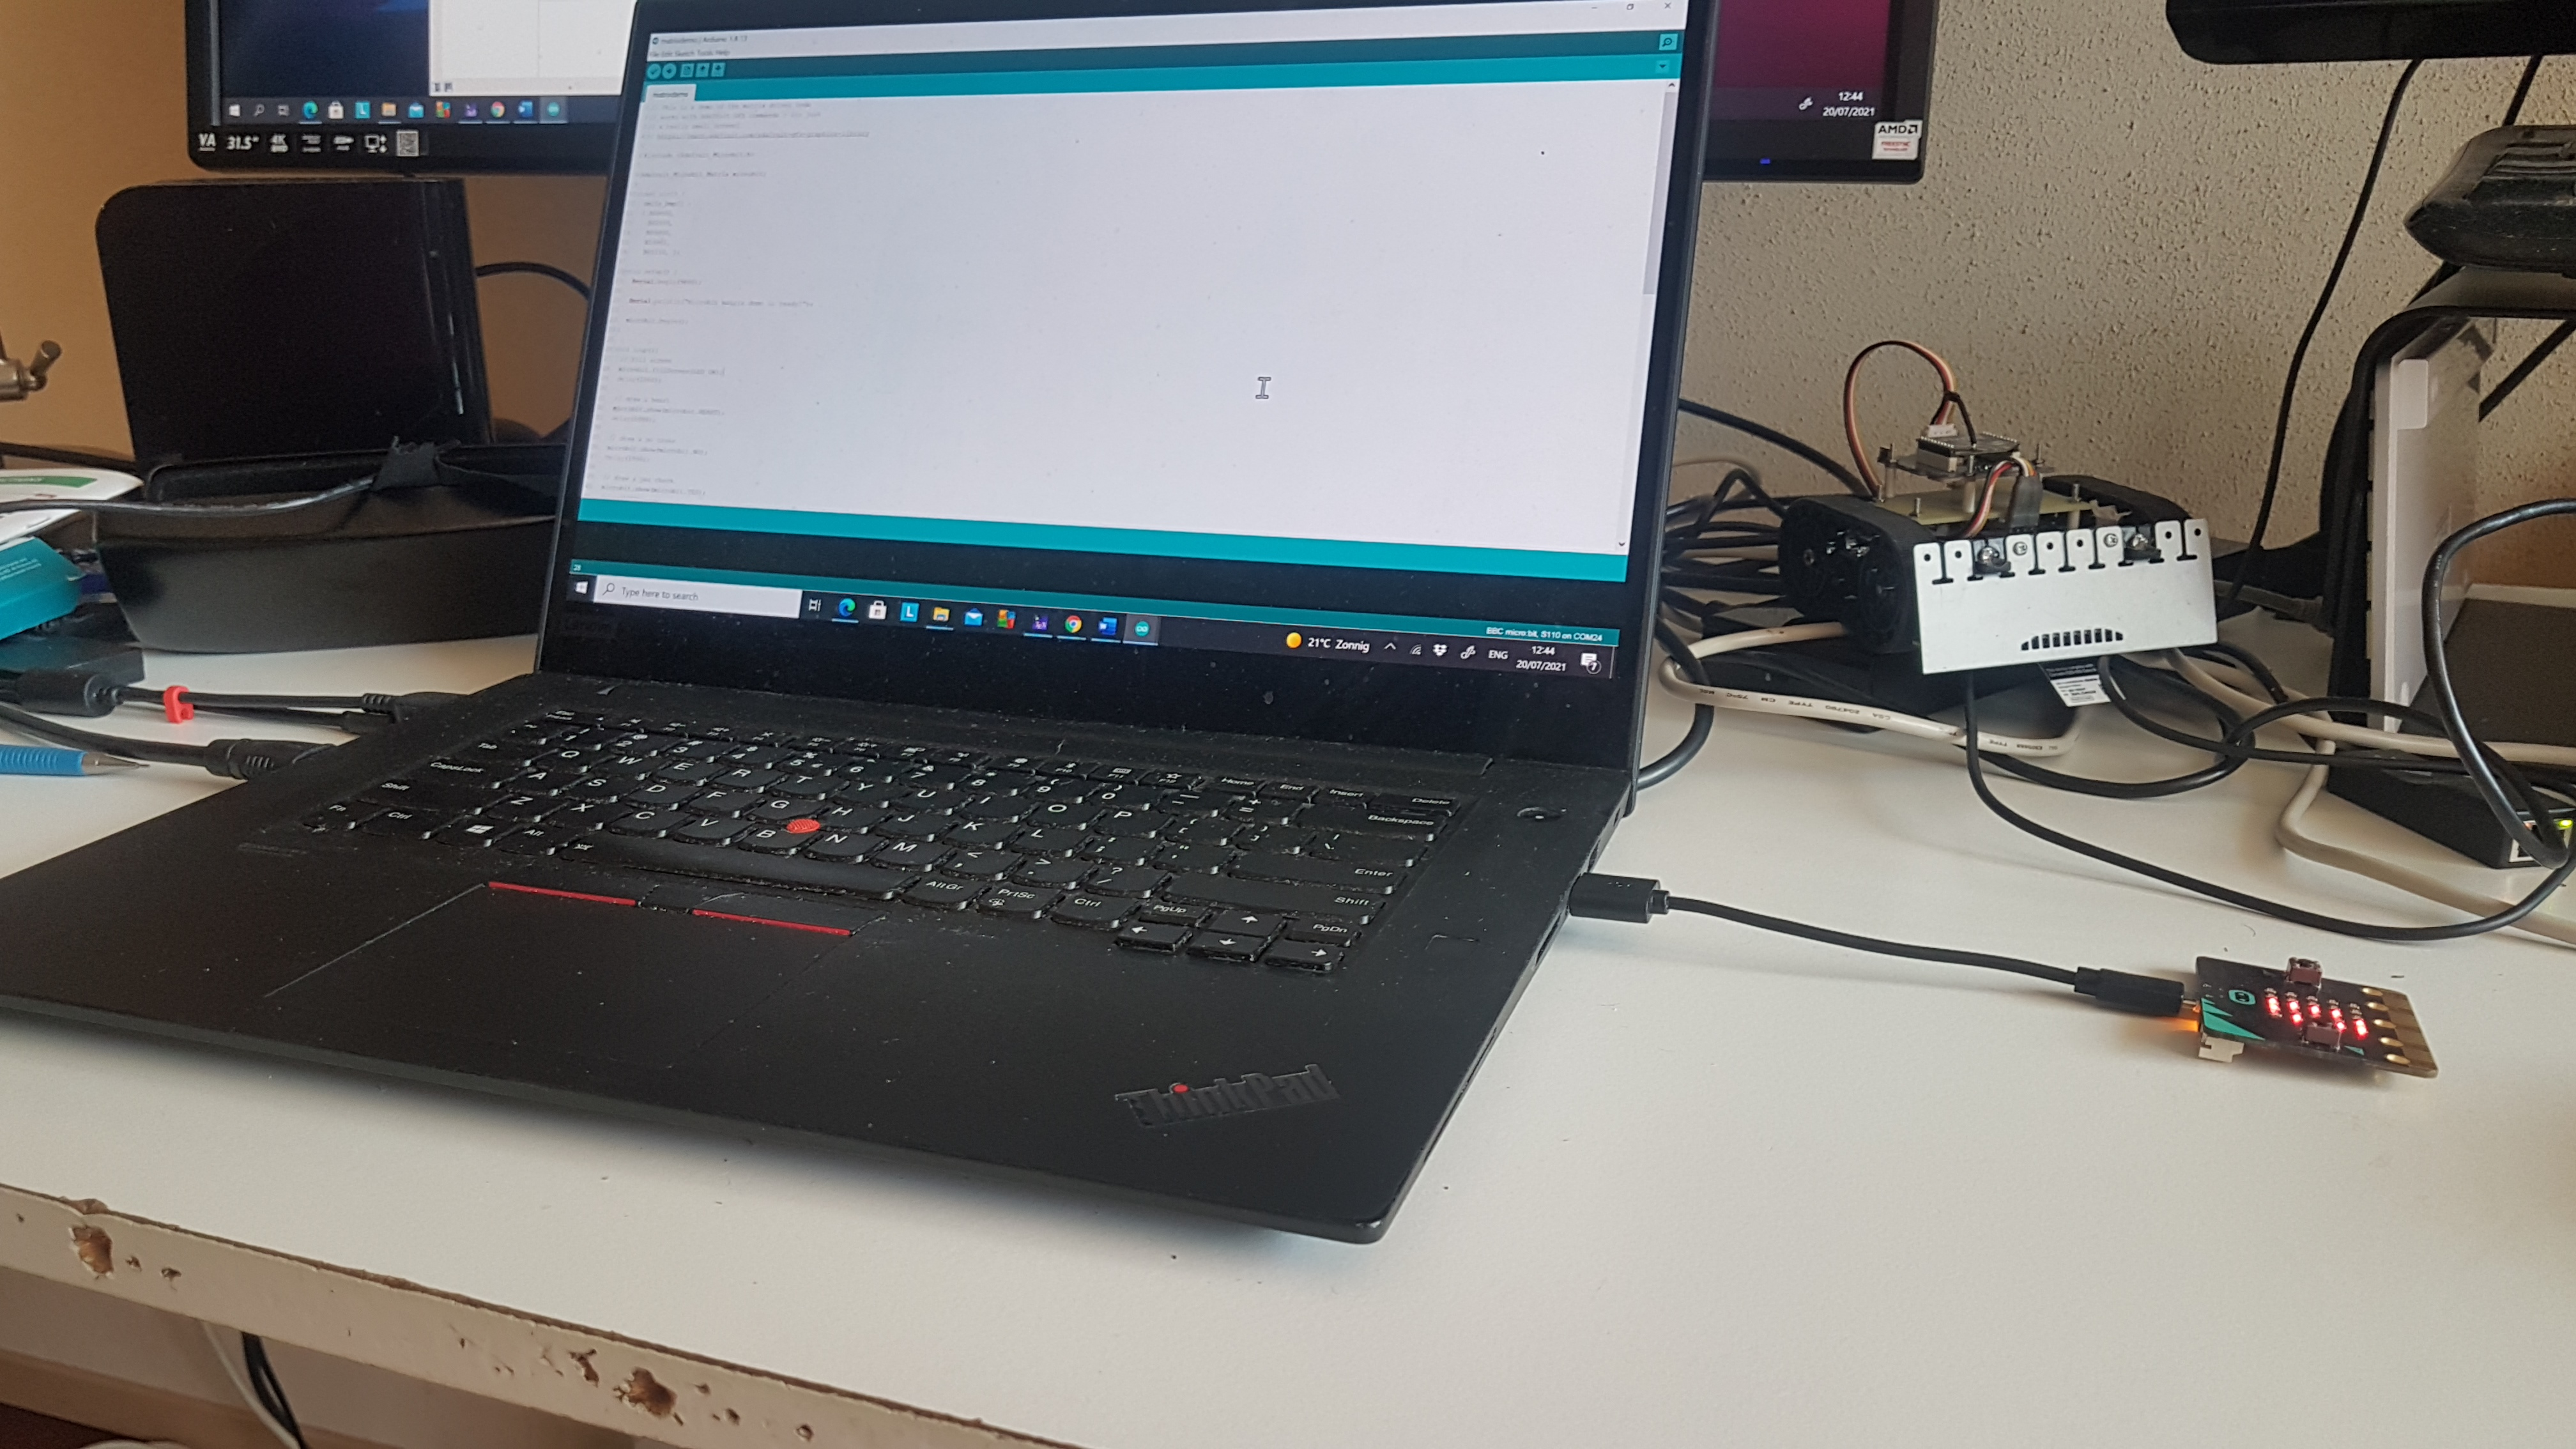
\includegraphics[width=0.40 \linewidth]{figuren/aansluitingBBC}
	\centering
	\caption{aansluiting van de BBC microbit.}
	\label{fig:aansluiting}
\end{figure}
Er zijn verschillende ontwikkelomgeving voor de BBC microbit, maar tijdens dit instructie college(practicum), zal voornamelijk via de \href{https://https://www.arduino.cc/en/software}{Arduino omgeving} omgeving gewerkt worden.


\section{Start met de BBC microbit}

De BBC Microbit is ontwikkeld om programmeeronderwijs te kunnen geven aan leerlingen van groep 7 (10/11-jarigen). Sinds 2016 wordt dit bordje aan elke groep 7 leerling verstrekt, elk jaar ongeveer 1 miljoen stuks. De hardware, het bordje is ‘open source’, de software die we er bij gebruiken ook.

De hardware is robuust, goedkoop, héél eenvoudig te programmeren, je kunt er veel mee en er is prima ondersteuning. Er zijn verschillende ontwikkel omgevingen gebruiken om programma’s te schrijven voor de Microbit. 

Je gaat de Microbit gebruiken in ‘The Challenge’. De Microbit is een Embedded System. Een Embedded System bestaat uit een microcontroller met sensoren en actuatoren. Met sensoren meet je iets (licht, temperatuur, beweging), met actuatoren stuur je iets aan (b.v een ledje, een speakertje, een motor, etc.). Met de Microbit kun je IoT (Internet of Things) devices simuleren, dit zijn ook Embedded Systems. Met een IoT device wordt meestal een apparaat bedoeld die een radiomodule bevat die data kan verzenden of ontvangen. Je kunt deze radiomodule zien als een black box. Er zijn veel verschillende typen voor veel verschillende toepassingen. Ze verschillen in bereik, datadoorvoer, reactiesnelheid en energieverbruik. 
Voor ‘The Challenge’ maakt het niet uit, je kunt met de Microbit prima een IoT device simuleren.

Let op: Het installeren van software moet je zelf uitzoeken, dit kost veel tijd. Verwacht daarom niet dat je docent je hiermee kan helpen!

Indien het niet lukt, kan altijd om hulp gevraagd worden, maar doe dat met specifieke vragen en vertelt erbij wat jezelf al uitgeprobeerd heb.


\subsection{Eerste kennismaking met de Microbit}

Sluit de microbit met behulp van een USB micro snoertje aan op je laptop, zoals te zien is in figuur \ref{fig:aansluiting}.
Windows herkent de microbit en kent daar een \textbf{drive letter} voor, zoals ook gebeurt bij een USB stick. Dit is te zien in figuur \ref{fig:driveL}.

\begin{figure}[h!]
	\captionsetup{justification=centering}
	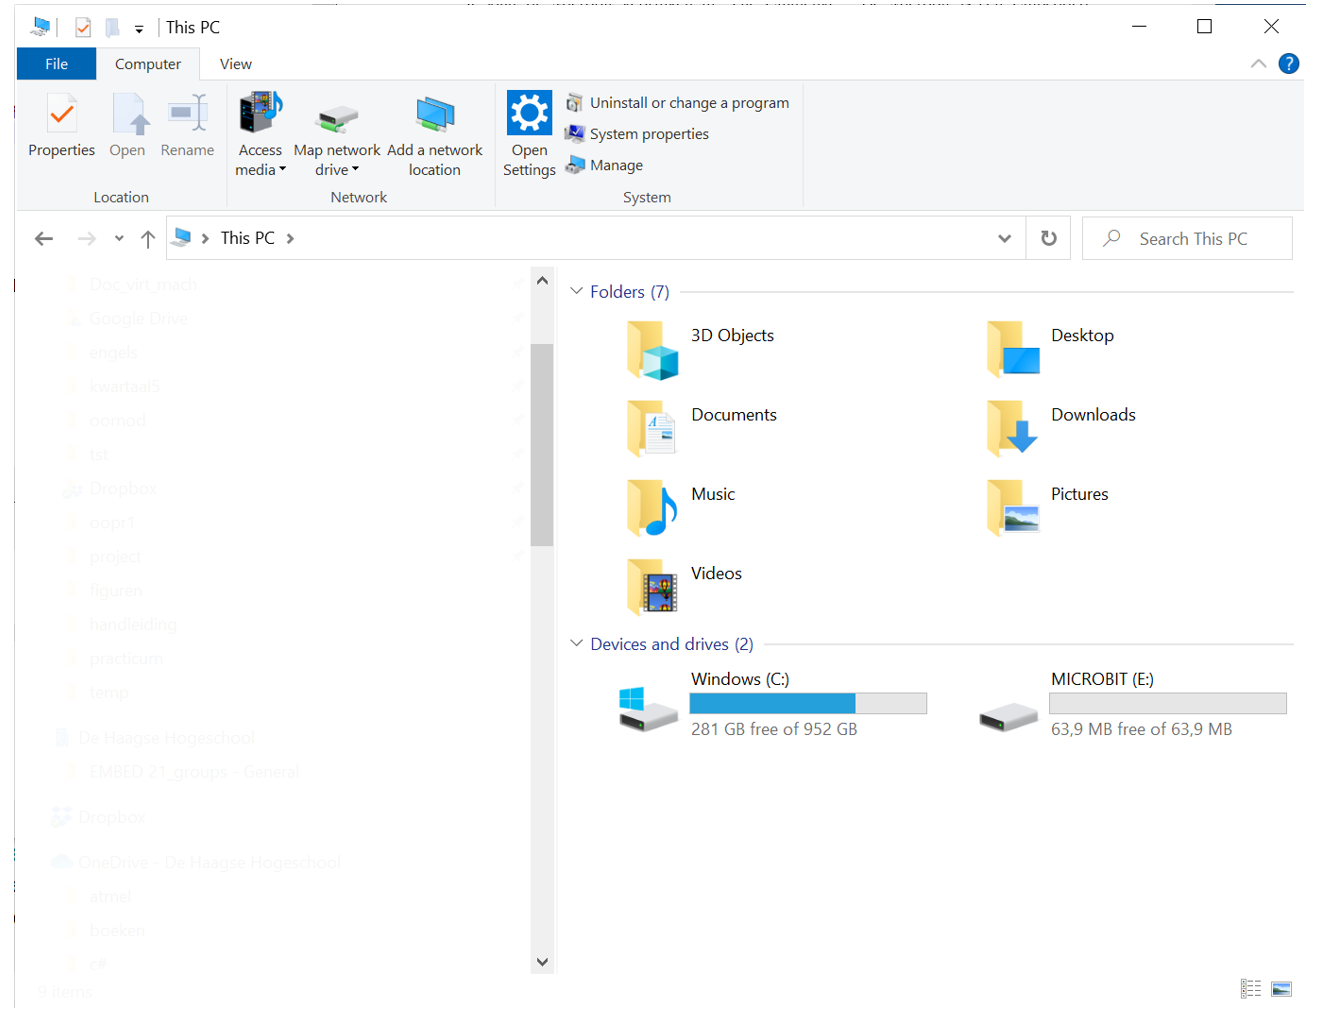
\includegraphics[width=0.50 \linewidth]{figuren/driverLetter}
	\centering
	\caption{Herkenning microbit in windows.}
	\label{fig:driveL}
\end{figure}

Na het aansluiten zal bij een nieuwe BBC microbit de ingebouwde demo gaan lopen. Werkt de ingebouwde demo niet, dan kan je naar de \href{https://support.microbit.org/support/solutions/articles/19000021613-reset-the-micro-bit-to-factory-defaults}{Reset de micro:bit to factory pagina} gaan en download het  \href{https://support.microbit.org/helpdesk/attachments/19067609189} {OutOfBoxExperience.hex} programma en zet dit op de MICROBIT drive. Hierdoor zal het programma geüpload worden op de microbit.

Voor verdere kennismaking met de microbit is de de pagina \href{https://microbit.org/get-started/first-steps/set-up/}{https://microbit.org/get-started/first-steps/set-up/}
een goed startpunt.

%Houd de kant met de twee knopjes naar je toe. Sluit de Microbit met een micro-USB kabel aan op je PC. De ledjes gaan knipperen, er komt tekst voorbij, volg de instructies.
%ls de Microbit eenmaal geprogrammeerd is, dan is het demoprogramma natuurlijk gewist. 
%Je kunt het originele demoprogramma OutOfBoxExperience-v2.hex (gemaakt in C++) hier downloaden: 

\subsection{De Microbit in “The Challenge”}

De doelstelling van The Challenge is dat hier producten van alle differentiaties in samenkomen. Voor het NSE/Embedded deel houden we het eenvoudig. Wat mij betreft is het prima om hier de “blokken” taal voor te gebruiken. Hier kun je alles mee.

Het ligt voor de hand dat NSE studenten in de Arduino omgeving programmeren, waar de programmeertalen C/C++ de voertaal is.

Voor een intro in de “blokken” taal, start hier en begin met ‘Mode’, ‘Step Counter’, kies voor ‘Instructies weergeven’: \href{https://makecode.microbit.org/}{https://makecode.microbit.org/}




\section{Kennismaken met de Arduino omgeving}

De Arduino omgeving oftewel Arduino IDE (Integrated Development Environment) kan je gebruiken om de Microbit te programmeren. 
%Mocht je de software nog niet geïnstalleerd hebben, volg dan de instructies in “Installatiehandleiding Arduino software voor BBC Microbit”.

We gebruiken de Arduino IDE omdat deze op beginnersniveau zeer veel gebruikt wordt en er veel voorbeeldcode te vinden is.
 
Eigenlijk maakt de Arduino IDE gebruik van de taal C++, dit is een Object Oriented uitbreiding van de taal C. Het C++ / Object Oriented deel van de programmeertaal zie je soms terug in instructies zoals Serial.begin(9600); De punt tussen Serial en begin is hier een indicatie van.

Java en C++ zijn object georiënteerde talen. Daarover leer je meer als je kiest voor de differentiaties “Software Engineering” of “Networks \& System Engineering”. Voor dit practicum houden we het eenvoudig. We gebruiken de taal zoveel mogelijk als klassieke “imperatieve” programmeertaal waarbij gewerkt wordt met een reeks opeenvolgende instructies.

%Voorheen maakten we gebruik van een Arduino Uno. We zijn overgestapt naar de Microbit omdat deze veel meer mogelijkheden biedt zoals meer ingebouwde sensoren en Bluetooth en ook nog eens goedkoper is dan een Arduino. 
%De Microbit is een IoT device (Internet of Things). Daardoor kun je in ‘The Challenge’ veel meer met een Microbit dan met een Arduino Uno.



\subsection{Het installeren van de Arduino omgeving}

VOER ONDERSTAANDE INSTALLATIE THUIS UIT – DIT DUURT 1,5 UUR!!!

\begin{enumerate}
	\item Download de Arduino software van \href{https://https://www.arduino.cc/en/software}{https://www.arduino.cc/en/software}, zoals je kan zien zijn er ook versies voor Linux en de Mac.
	\item Kies de Windows installer, niet de app. De app is niet geschikt voor wat wij gaan doen.
	\item  Bevestig alle vragen, klik maar door.
\end{enumerate}

Instellingen wijzigen: Ga naar File $\rightarrow$ Preferences $\rightarrow$ Sketchbook location, zoals te zien in figuur \ref{fig:arduinoPref}, en wijzig het pad:
\begin{figure}[h!]
	\captionsetup{justification=centering}
	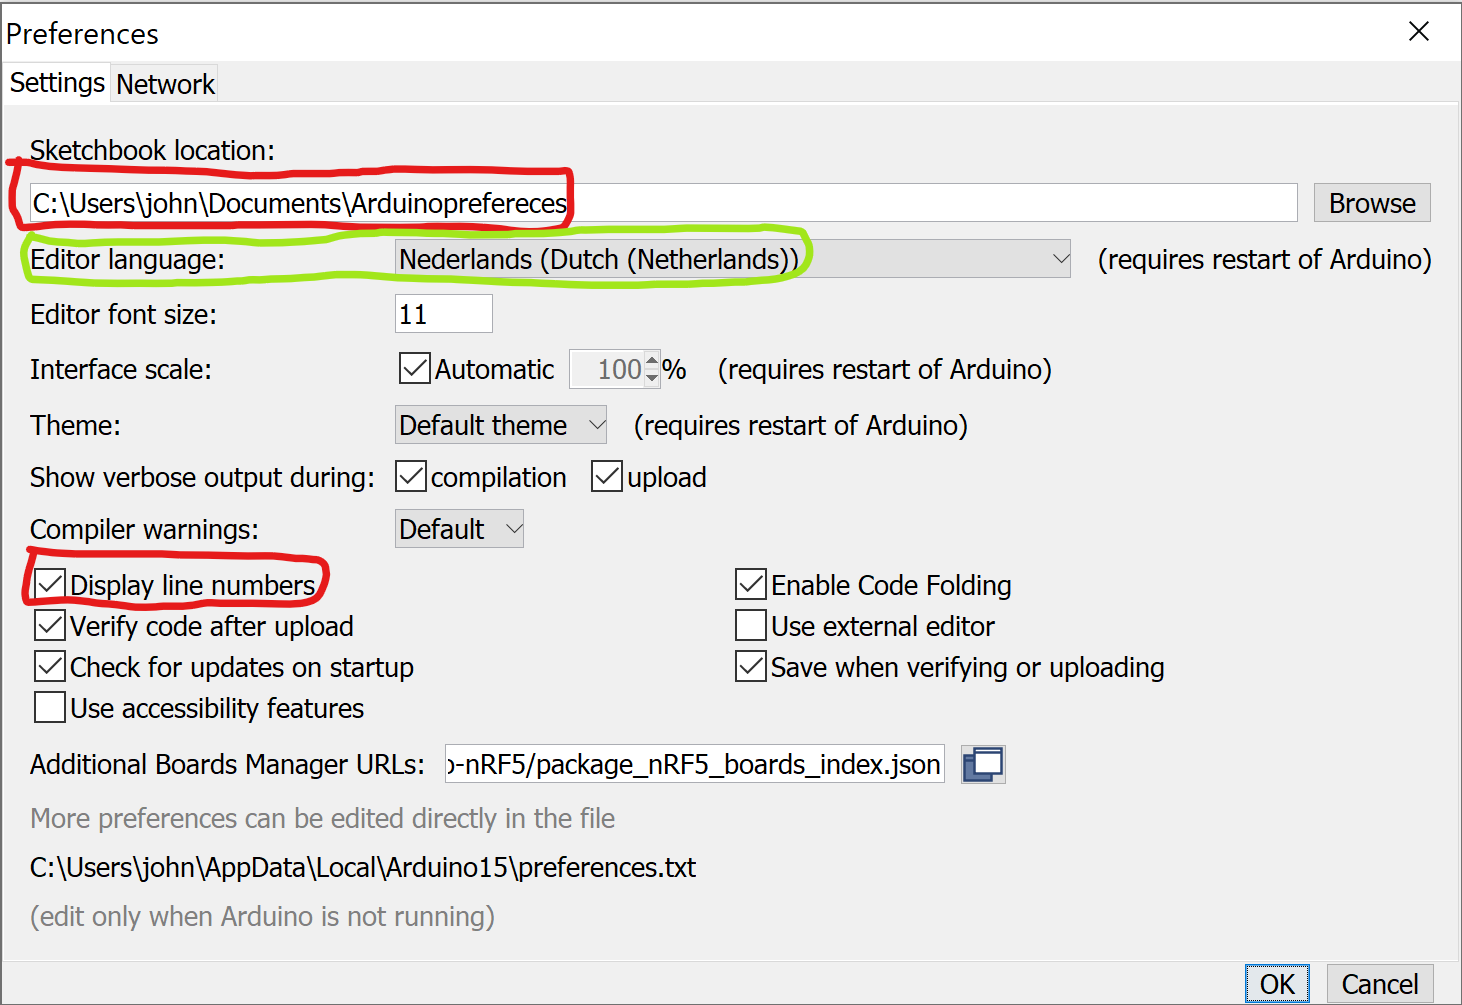
\includegraphics[width=0.50 \linewidth]{figuren/arduinoPref}
	\centering
	\caption{preferences scherm.}
	\label{fig:arduinoPref}
\end{figure}

\begin{itemize}
	\item C:\textbackslash Users\textbackslash \textit{john}\textbackslash Documents\textbackslash Arduino (in mijn geval)
	\item Zet “Display line numbers” aan.
	\item Indien de Arduino omgeving Engelstalig is, kan deze gewijzigd worden naar het Nederlands. Het is handig om tijdens de installatie de Engelstalige omgeving te gebruiken.
\end{itemize}


\subsection{De arduino omgeving geschikt maken voor de microbit.}

De firma \href{https://www.adafruit.com/about}{Adafruit } ontwikkelt diverse componenten voor met name embedded systemen
die door ieder gebruiker kan worden toegepast en/of geprogrammeerd. Om dit waar te kunnen maken worden veel tutorials ontwikkeld. Zo is er ook een uitgebreide website, om de \href{https://learn.adafruit.com/use-micro-bit-with-arduino}{microbit met de Arduino IDE} te programmeren.
\begin{enumerate}
	\item Ga naar de Adafruit website om  de \href{https://learn.adafruit.com/use-micro-bit-with-arduino}{microbit met de Arduino IDE} te programmeren.
	\item Scroll naar beneden en klik op \fcolorbox{black}{NavyBlue}{\textcolor{White}{\textbf{Install board and blink! \textgreater}}}. Voer vervolgens het onderdeel "Add NRF5x Board Support" uit (dit kan een enige tijd duren, raak niet in paniek en neem wat te drinken). Nadat de installatie gebeurd is wordt dit door Adafruit uitgetest met het programmaatje blink. Het werken met het programma blink wordt gedaan bij punt \ref{en:blink}.
	
	\item Het selecteren van de BBC micro:bit V2 board en de USB port.
	\begin{enumerate}
		\item Selecteer BBC micro:bit V2.
		\begin{figure}[h!]
			\captionsetup{justification=centering}
			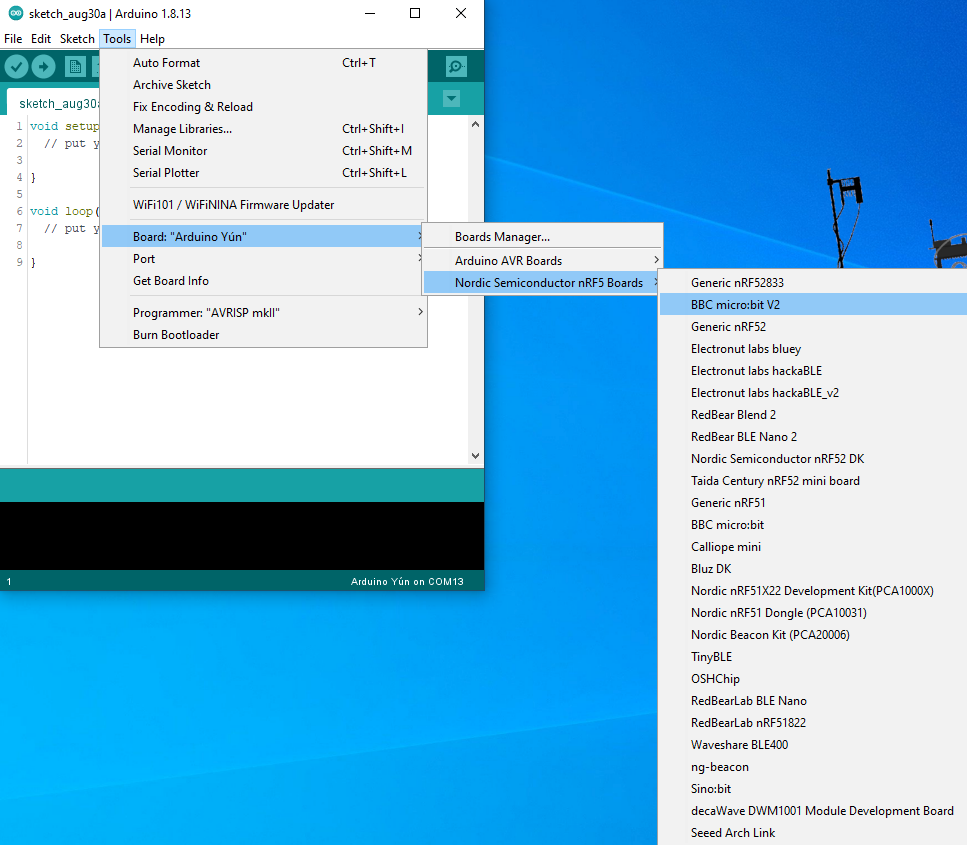
\includegraphics[width=0.45 \linewidth]{figuren/selBBCV2}
			\centering
			\caption{Selecteren van de BBC micro:bit V2.}
			\label{fig:selBoard}
		\end{figure}
	    \item Het setten van de USB port.
	     	\begin{figure}[h!]
	     	\captionsetup{justification=centering}
	     	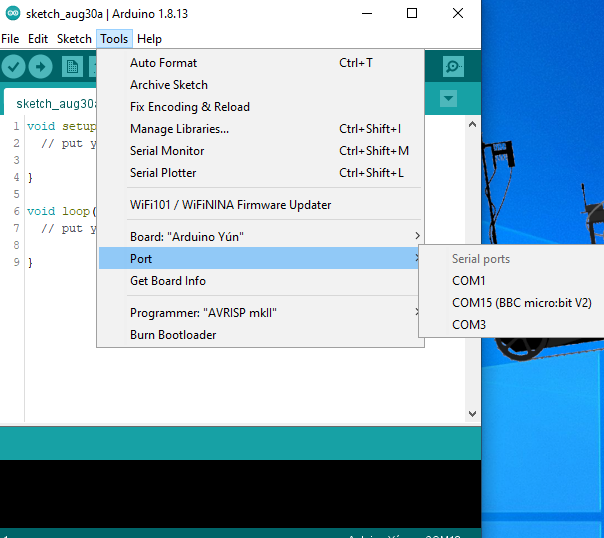
\includegraphics[width=0.45 \linewidth]{figuren/selBBCPort}
	     	\centering
	     	\caption{Selecteren van de USB port.}
	     	\label{fig:selUSB}
	     \end{figure}
     Indien de microbit niet herkent wordt, start de arduino omgeving opnieuw op en/of plug de microbit opnieuw in de USB poort.
	\end{enumerate}
~ 
   \item Het uploaden van een programma gebeurt door op de knop \img{figuren/ardIcUpl} te klikken. Windows komt met de melding zoals hieronder wordt weergegeven. 
   	\begin{figure}[h!]
   	\captionsetup{justification=centering}
   	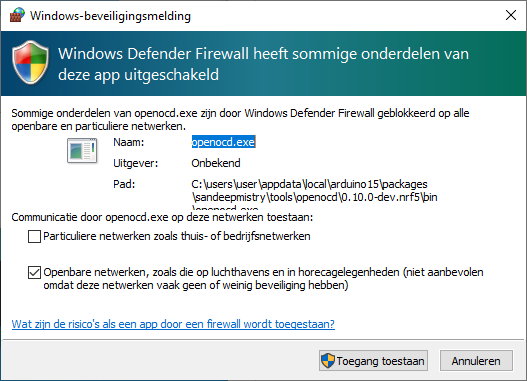
\includegraphics[width=0.45 \linewidth]{figuren/windowsDefSec}
   	\centering
   	\caption{Melding van windows defender.}
   	\label{fig:windowsDef}
   \end{figure}
Hiermee vraagt Windows toestemming om de USB port te mogen gebruiken.
\item Haal de voorbeeldcode van blackboard of \href{http://home.caiway.nl/~johnvi/embeddedFirstSem/voorbeeldCodeEmbedded.zip}{download} de laatste versie en plaats deze in je eigen werkdirectory.
\item \label{en:blink} Open het voorbeeldprogramma blink.ino (dubbel klik), dat wordt weergegeven in Listing \ref{lst:blink}, compileer en upload naar de micro:bit (klik op de knop \img{figuren/ardIcUpl}). \\
Als het goed is gaat het linkerboven LEDje van de matrix knipperen.

\end{enumerate}




